\section{Background and Related Work}

\begin{figure}[!ht]
  \centering
  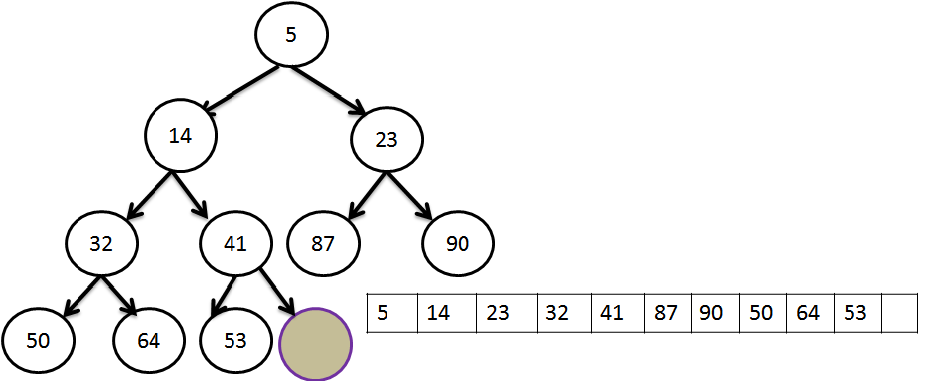
\includegraphics[width=7cm]{fig/fig2.png}
      \caption{Binary min heap with its array representation.}
    \label{fig2}
\end{figure}

A priority queue is a data structure that maintains a collection of elements using the following set of operations by a minimum priority queue $Q$:
\begin{itemize}
\item {\bf Insert:} Insert a number into $Q$, provided that the new list should maintain the priority queue.

\item {\bf Min-delete:} Find the minimum number in $Q$ and delete it from $Q$. After deletion, the property of priority queue should be kept unchanged.
\end{itemize}


%\subsubsection{Priority Queue Implementation}
A priority queue can be implemented by using a binary heap data structure.
%\begin{definition}
A min-heap is a complete binary tree $H$ such that the data contained in each node is less than or equal to the data in that node's children.
%\end{definition}
Figure \ref{fig2} shows the binary min heap $H$.
The root of $H$ is $H[1]$.
Given the index $i$ of any node in $H$, the indices of its parent and children can be determined in the following way:
\begin{eqnarray*}
parent[i] &=&  \lfloor i/2 \rfloor \\
leftChild[i] &=& 2i\\
rightChild[i] &=& 2i + 1
\end{eqnarray*}

The {\it insert} algorithm on the binary min heap $H$ is as follows:
\begin{enumerate}
\item Place the new element in the next available position e.g. $i$ in $H$.
\item Compare the new element, $H[i]$, with its parent, $H[i/2]$. If $H[i]$ $<$ $H[i/2]$, then swap their values.
\item Continue this process until either the new element's parent is smaller than or equal to the new element, or the new element reaches the root, $H[1]$.
\end{enumerate}

\begin{figure}[!ht]
  \centering
  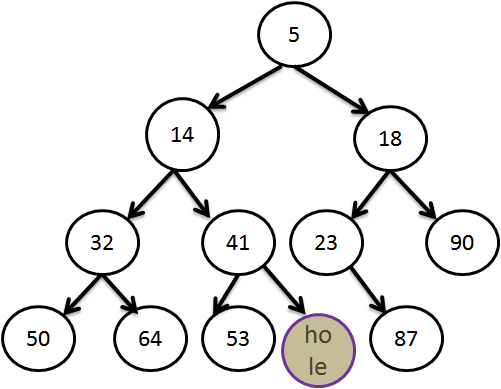
\includegraphics[width=4cm]{fig/fig3.png}
      \caption{New heap structure after inserting $18$.}
    \label{fig3}
\end{figure}

\begin{figure}[!ht]
  \centering
  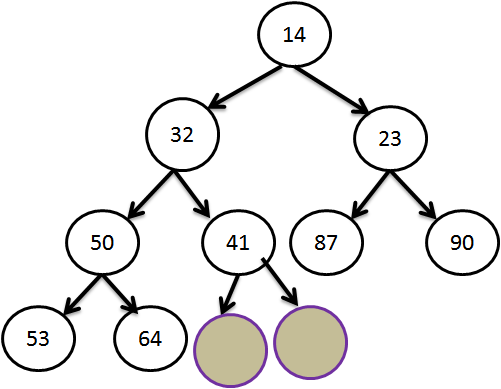
\includegraphics[width=4cm]{fig/fig4.png}
      \caption{New heap structure after a delete operation from the original heap shown at Figure \ref{fig2}.}
    \label{fig4}
\end{figure}

Figure \ref{fig3} shows the new heap structure after inserting $18$ into the original heap from Figure \ref{fig2}.

The {\it min-delete} algorithm is as follows:
\begin{enumerate}
\item Return root element, $H[1]$.
\item Replace the root with the last element at the last level e.g. $H[i]$.
\item Compare the new root with its children. Unless the root is smaller than its children, swap the root and its min child.
\item Continue swapping for each level by comparing $H[i]$ with $H[2i]$ and $H[2i+1]$, until the parent becomes less than its children or reaches to the leaf node.
\end{enumerate}

Figure \ref{fig4} depicts the heap structure after a min-delete operation on the original heap shown at Figure \ref{fig2}.
We can see that $5$ was the previous root element at Figure \ref{fig2}.
The heap is restructured according to the min-delete algorithm.

\subsection{Pipelined Binary Heap}
As a binary heap accumulates more levels of nodes due to insertions, processing incoming operations becomes slower.
This slowdown can be avoided by pipelining operations in the heap.
Multiple operations can then be handled in parallel, resulting in a speedup.

To clarify using an example, suppose a pipelined binary heap receives a sequence of two {\it inserts}, and the last level can hold two more elements.
These two indices share the same parent index.
Assume that the placement of a new element and the comparison with swapping each take a clock cycle.
Upon encountering the first operation, the new element is inserted at the last level.
While the first inserted element is compared to its parent and swapped if necessary, the element from the second operation is inserted.
The second element is compared and potentially swapped with the (updated) parent, while the first element is handled at the next level.
From this example, a pipelined binary heap can ideally process one operation at each level.

Difficulties arise when processing insert and delete operations in parallel.
{\it Inserts} and {\it min-deletes}, in normal cases, start at the last and first level of the heap respectively and progress their tasks in opposite directions.
Moreover, insert-delete combinations can create {\it holes} in the heap. 
A hole occupies a node in the heap, but it does not contain valid data.
Though holes unnecessarily increase the depth of the heap, which delays response time for further operations, but the most significant negative impact is that they waste storage resources.
Existing hardware-based pipelined heaps, to be discussed in related work, do not have any method to refill a hole.
In the worst-case scenario, shown in Figure \ref{hole}, hardware cost double. 
We discuss more about parallel insert-delete operations and holes in Section III.

\begin{figure}[!ht]
  \centering
  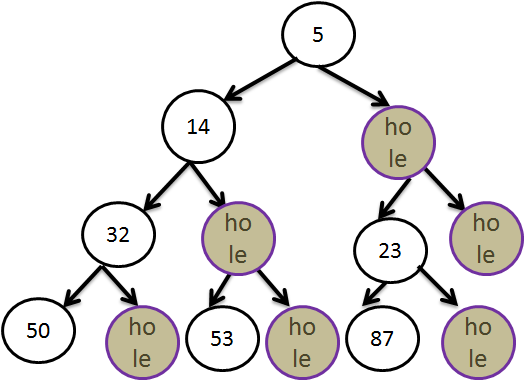
\includegraphics[width=4cm]{fig/hole.png}
      \caption{Worst-case scenario for hole creation.}
    \label{hole}
\end{figure}

\subsection{Related Work}
Several authors have theoretically proven that the parallel heap is an efficient data structure for implementing a priority queue.
Prasad {\it et. al.} \cite{pq3} theoretically illustrate that this data structure requires $O(p)$ operations with $O(\log n)$ time for $p \leq n$, where $n$ is the number of nodes and $p$ is the number of processors used.
This idea is designed for the EREW PRAM shared memory model of computation.
The many-core architecture by \cite{pq2} in GPGPU platform provides multi-fold speedup.
Another theoretical approach \cite{pq4} deploys a pipeline or tree of processors ($O(\log n)$, where $n$ is the number of nodes).
The implementation of this algorithm \cite{pq5} is expensive for multi-core architectures.

%\subsubsection{Hardware Based Priority Queue}
There have been several hardware-based priority queue implementations described in literature \cite{hw1,hw2,hw3,hw5,hw6,hw7,hw8,hw9}.
Pipelined hardware implementations can attain $O(1)$ execution time \cite{hw5,hw6}.
However, due to several limitations such as cost and size, most hardware implementations do not support a large number of nodes to be processed.
Thus, these implementations are limited in scalability.
%In \cite{hw7}, the author claims that the pipelined heap is the most efficient implementation.  However, this implementation incurs high hardware cost. The design is not flexible, more specifically, it is designed with a fixed heap size.
The {\it Systolic Arrays} and the {\it Shift Registers} \cite{hw8,hw9} based hardware implementations are well known in literature.
The common drawback of these two implementations is the usage of a large number of comparators ($O(n)$).
These comparators are responsible for comparing nodes from different levels with $O(1)$ step complexity.
For the {\it Shift Register} \cite{hw9} based implementations, when new data comes for processing, it is broadcasted to all levels.
This requires global communicator hardware, which connects to all levels.
The implementation based on {\it Systolic Arrays} \cite{hw8} needs a larger storage buffer to hold preprocessed data.
These approaches are not scalable, and they require $O(n)$ comparators for $n$ nodes.
To overcome the hardware complexity, \cite{hw10} implements a recursive processor where hardware use is drastically reduced by compromising execution time.
Bhagwan and Lin \cite{hw2} design a physical heap such that commands can be pipelined between different levels of the heap.
The authors in \cite{hw1} give a pragmatic solution of the {\it fanout} problem mentioned in \cite{hw3}.
The design presented in \cite{hw11} is very efficient in terms of hardware complexity but very slow in execution ($O(\log n$)), as it is implemented using hardware-software co-design.

For the FPGA-based priority queue implementation, Kuacharoen {\it et. al} \cite{fpga3} implement the logic presented in \cite{hw3} by incorporating extra features to ensure that the design would act as a real-time operating system task scheduler.
The major limitation of this work is that it deals with very few priority levels and a small number of items in the queue at any given time.
A hybrid priority queue is implemented by \cite{fpga2}, and it ensures high scalability and high throughput.
The ASIC-based pipelined heap presented by Ioannou {\it et. al} \cite{fpga1} is scalable and can run for 64K nodes without compromising performance, but it takes at least three clock cycles in the average case to complete a single stage.
Kumar {\it et. al} \cite{hwsw1} propose a new hybrid priority queue architecture that can be managed in hardware and/or software.
The main drawback is that it operates on $O(\log n)$ time.

However, all aforementioned designs never address the {\it holes} created from parallel {\it insert-delete} operations (an insert operation followed by a min-delete operation).
In the next section, we present our proposed design with hole minimization, including several optimization techniques for performance efficiency and hardware minimization.
